\documentclass[12pt,a4paper]{article}
\usepackage[utf8]{inputenc}
\usepackage[english]{babel}
\usepackage[english]{isodate}
\usepackage[parfill]{parskip}
\usepackage{fancyhdr}
\usepackage{hyperref}
\usepackage[os=win]{menukeys}
\usepackage{graphicx}
\graphicspath{ {./images/} }
\usepackage{cleveref}
\usepackage{fancyhdr}
\pagestyle{fancy}
\fancyhead[L]{\rightmark}
\fancyhead[R]{\textbf{\thepage}}
\renewcommand{\sectionmark}[1]{\markright{\thesection\quad#1}}
\setlength{\headheight}{15pt}
\begin{document}
\renewcommand{\familydefault}{\sfdefault}
\sffamily
\begin{titlepage}
    \begin{center}
        \vspace*{1cm}

        \Huge
        \textbf{Doomfist Parkour Mapmaking Guide}

        \vspace{0.5cm}
        \Large
        Hax Framework User Manual
            
        \vspace{1.5cm}

        \textbf{Written by \\
        thecyberon}
        
        \vfill
            
        Edited by nebula
            
        \vspace{0.8cm}
    
            
    \end{center}
\end{titlepage}
\tableofcontents
\pagenumbering{arabic}
\newpage
\section{Preface}

    This guide aims to reach out to as many people as I can, including total beginners who want to 
embark on their own Doomfist Parkour multilevel map making journey. If you currently know 
nothing about multilevel map making and want a step-by-step walkthrough on how to make your 
own multilevel map, here’s the right place to be at. If you already know some stuff or some 
basics about multilevel mapmaking, you may find this guide to be slightly long winded (since it 
is targeted to cover a large target audience of people who know almost nothing about multilevel 
map making); you can narrow down to the parts that you wish to learn and hopefully you’d be 
able to find some useful tips and tricks within the guide. 

Also, do note that this guide is written to cover 
information up to
v.1.9.1 of Hax Framework.
Credit goes to to Hax for coming up with this awesome framework.

For more specific help and discussion join the Doomfist Parkour Discord community at \url{discord.gg/doomfistparkour}

\textit{Disclaimer: I don’t know 100\% of the tools and settings here. However, the good news is you 
don’t need to know every command, every code and every rule in the workshop to create your 
own map. You just need to know some of the useful stuff and you’re good to go. Have fun!}

\newpage
\section{Creating a Mapmaking Lobby}
    
    \subsection{Setting up}
        Beginning at the Overwatch main menu, create a custom lobby by clicking on the following buttons:\\ \\
        \centerline{\menu[,]{Play, Game Browser, Custom Game, Create, Settings}}\\ \\
        Remember, you can hover over a button to see what it is.
        Your screen should look like \cref{fig:Picture1}.
    
        \begin{figure}[ht]
            \centering
            \includegraphics[width=\textwidth,height=\textheight,keepaspectratio]{Picture1.png}
            \caption{\keys{Import Code} and map choice button locations}
            \label{fig:Picture1}
        \end{figure}
    
        Click on \keys{Import Code}, the second button from the left below the \textbf{SUMMARY} header on the right side of the screen (\cref{fig:Picture1}). Type ``\textit{HAVVX}'' (not case-sensitive) when prompted. Then, go to \keys{Maps} (left corner of the screen, below Presets \cref{fig:Picture1}), and select the map that you want. Remember to check that every other map selection is set to \textbf{OFF}, \emph{except} for the map that you want to work on, which will be set to \textbf{ON} (\cref{fig:Picture2}). If you want to work on a map that has variants, for example, \emph{Eichenwalde} vs \emph{Eichenwalde Halloween}, remember to select the correct variant as they are different from each other.
        
        \begin{figure}[ht]
            \centering
            \includegraphics[width=\textwidth,height=\textheight,keepaspectratio]{Picture2.png}
            \caption{Map selection page}
            \label{fig:Picture2}
        \end{figure}
        
        \begin{figure}[ht]
            \centering
            \includegraphics[width=\textwidth,height=\textheight,keepaspectratio]{Picture4.png}
            \caption{Workshop Settings button}
            \label{fig:Picture4}
        \end{figure}
        \clearpage
    
    \subsection{Workshop Settings}
        Access these settings by clicking the orange \keys{Workshop Settings} button shown in \cref{fig:Picture4}.
        
        \begin{figure}[ht]
            \centering
            \includegraphics[width=\textwidth,height=\textheight,keepaspectratio]{Picture5.png}
            \caption{Workshop Settings page}
            \label{fig:Picture5}
        \end{figure}
        
        \textbf{Multiple Creators}
        
        If you are making your map with another friend, you can invite them to the lobby and work on the map together! In order to enable this feature, you must ensure that \textit{MULTIPLE CREATORS} is set to \textbf{ON} (\cref{fig:Picture5}). You can have up to eight creators.
        
        \textbf{Checkpoint Skipping Speed}
        
        Changing \textit{SKIP/GO BACK SPEED} allows you to alter the time it takes to skip forward or back between checkpoints.
        
        \textbf{Automatically Skip to Newly Created Checkpoints}
        
        Setting \textit{MOVE TO THE CREATED CHECKPOINT} to \textbf{ON} will automatically bring you to the checkpoint you just created. Conversely, leaving this setting off will keep you in your original location.
        
        \textbf{Element Limiter (WARNING! Advanced creators only!)}
        
        This framework only allows four elements for each checkpoint. Elements include the connected checkpoints and any type of orb or light shaft. To use this option, you first need to enable the ``\textit{Play More Effects}'' option in the ``\textit{Edit Extensions}'' menu. In order to enable that option, you can gain ``\textit{Extension Points}'' by removing player slots. Doing this will double the amount of effects that can be shown at the same time.
        
        This setting will remove the limit of four elements allowing you to add as many elements as you'd like. This may lead to unintended issues with the map you are creating such as effects not rendering.
    
    \subsection{Starting the lobby}
        Now that you have finished setting up the lobby, you can use the \keys{Start} button in the ``\textit{Lobby}'' menu (\cref{fig:Picture3}). It is recommended to set the lobby to ``\textit{Invite Only}'' so that you can work on your map privately.
        \begin{figure}[ht]
            \centering
            \includegraphics[width=\textwidth,height=\textheight,keepaspectratio]{Picture3.png}
            \caption{Custom Game Lobby menu}
            \label{fig:Picture3}
        \end{figure}
\newpage
\section{Mapmaking}
    There are two main types of parkour maps: \emph{Multilevel} and \emph{Diverge/Single}.
    
    \textbf{Multilevel} is the default type and it allows for a initial checkpoint where you can select a specific level.  Another name for this initial checkpoint would be \emph{Level Select}.
        
    \textbf{Diverge/Single}, as the name suggests, does not allow for multiple levels.
    
    \subsection{Creating a Level Select or a Single Level}
        
        You are able to create as many levels as the workshop allows. This number is not known but it is best to not come close to that limit as the map may become unstable and crash unexpectedly, so just be wary.
        
        \begin{figure}[ht]
            \centering
            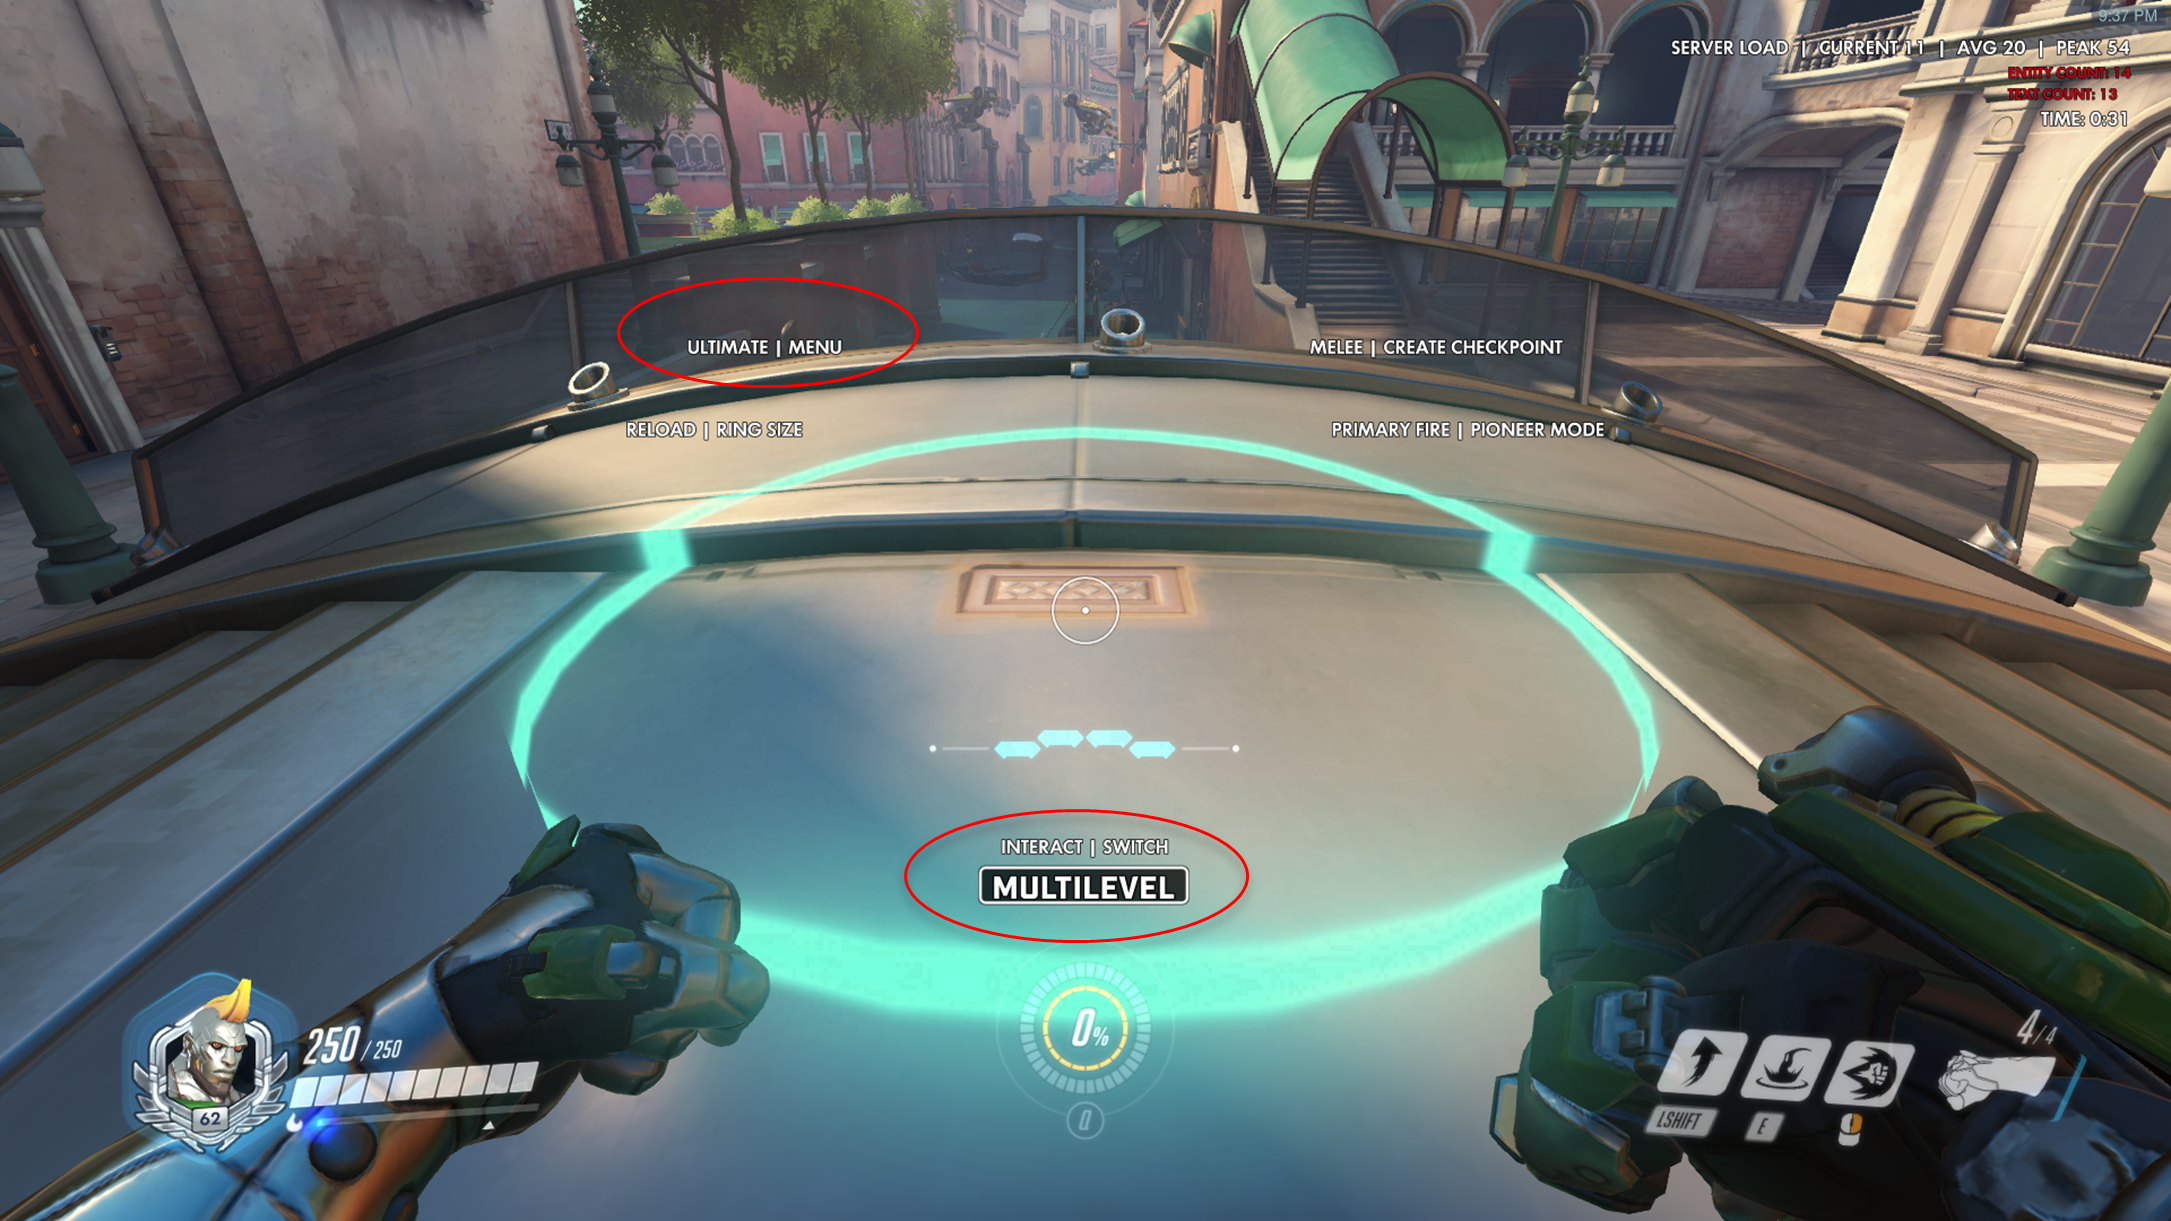
\includegraphics[width=\textwidth,height=\textheight,keepaspectratio]{Picture6.png}
            \caption{Multilevel/Diverge toggle and Menu button}
            \label{fig:Picture6}
        \end{figure}
        
        Take your time to explore and find a good place to start. \textit{(Tip: An example of a good starting point will be here on the bridge, where you can travel in many different directions and places using your abilities as Doomfist.} As seen in \cref{fig:Picture6}, if you press \keys{INTERACT}, you can switch between the multilevel and diverge modes.
        
        Once you have chosen a good starting point for yourself, position your cursor well and press \keys{MELEE}. \emph{This will now be your starting point.}

        \textit{(Note: I recommend deciding on the number of levels you wish to make and the respective entry 
            points into these levels before actually starting work on any levels, it helps you to plan and it 
            gives you a good sense of direction.)}  
    
    \subsection{Menu Navigation}
        Refer to the necessary figures for each menu item that is listed in this guide. The buttons required will be displayed in the menu. To go back to the last menu, press \keys{ULTIMATE}. 
    
    \subsection{Abilities, View Angles, and Recenter Menu}
        \subsubsection{Ability enable/disable}
            Before you make the level starting checkpoints, you may wish to determine the abilities that 
            you want to allow. You can leave all enabled; however, sometimes you may want to 
            disable a particular ability (e.g. \emph{Uppercut}) and allow players to only use \emph{Punch} and \emph{Slam} at 
            the level selection phase.
            Assuming you want to disable certain abilities (e.g. \emph{Uppercut}) at the level selection phase, here 
            are the steps to follow (\cref{fig:Picture7,fig:Picture8})
            \begin{enumerate}
              \item Press \keys{ULTIMATE} to access the menu. The option at the top left corner of 
                    your framework menu (\cref{fig:Picture6}).
              \item Press \keys{PRIMARY FIRE} to access the ability enable/disable menu (\cref{fig:Picture7}).
              \item At the bottom right-hand side of your screen, you can see which abilities are currently 
                    enabled (\cref{fig:Picture8}). For example, if you do not want to allow \emph{Uppercut}, you can 
                    press \keys{ABILITY 1} (on PC this is \keys{SHIFT}). If you change your mind and want to allow uppercut to be used again, 
                    press \keys{ABILITY 1} once more. \emph{Abilities that are allowed will be shown normally, abilities that 
                    are disabled will be in red}. In \cref{fig:Picture8}, you can see that \emph{Uppercut} is disabled, only 
                    \emph{Punch} and \emph{Slam} are enabled. Use the corresponding buttons for each ability to enable or disable them. 
    
            \end{enumerate}
    
        \begin{figure}[ht]
            \centering
            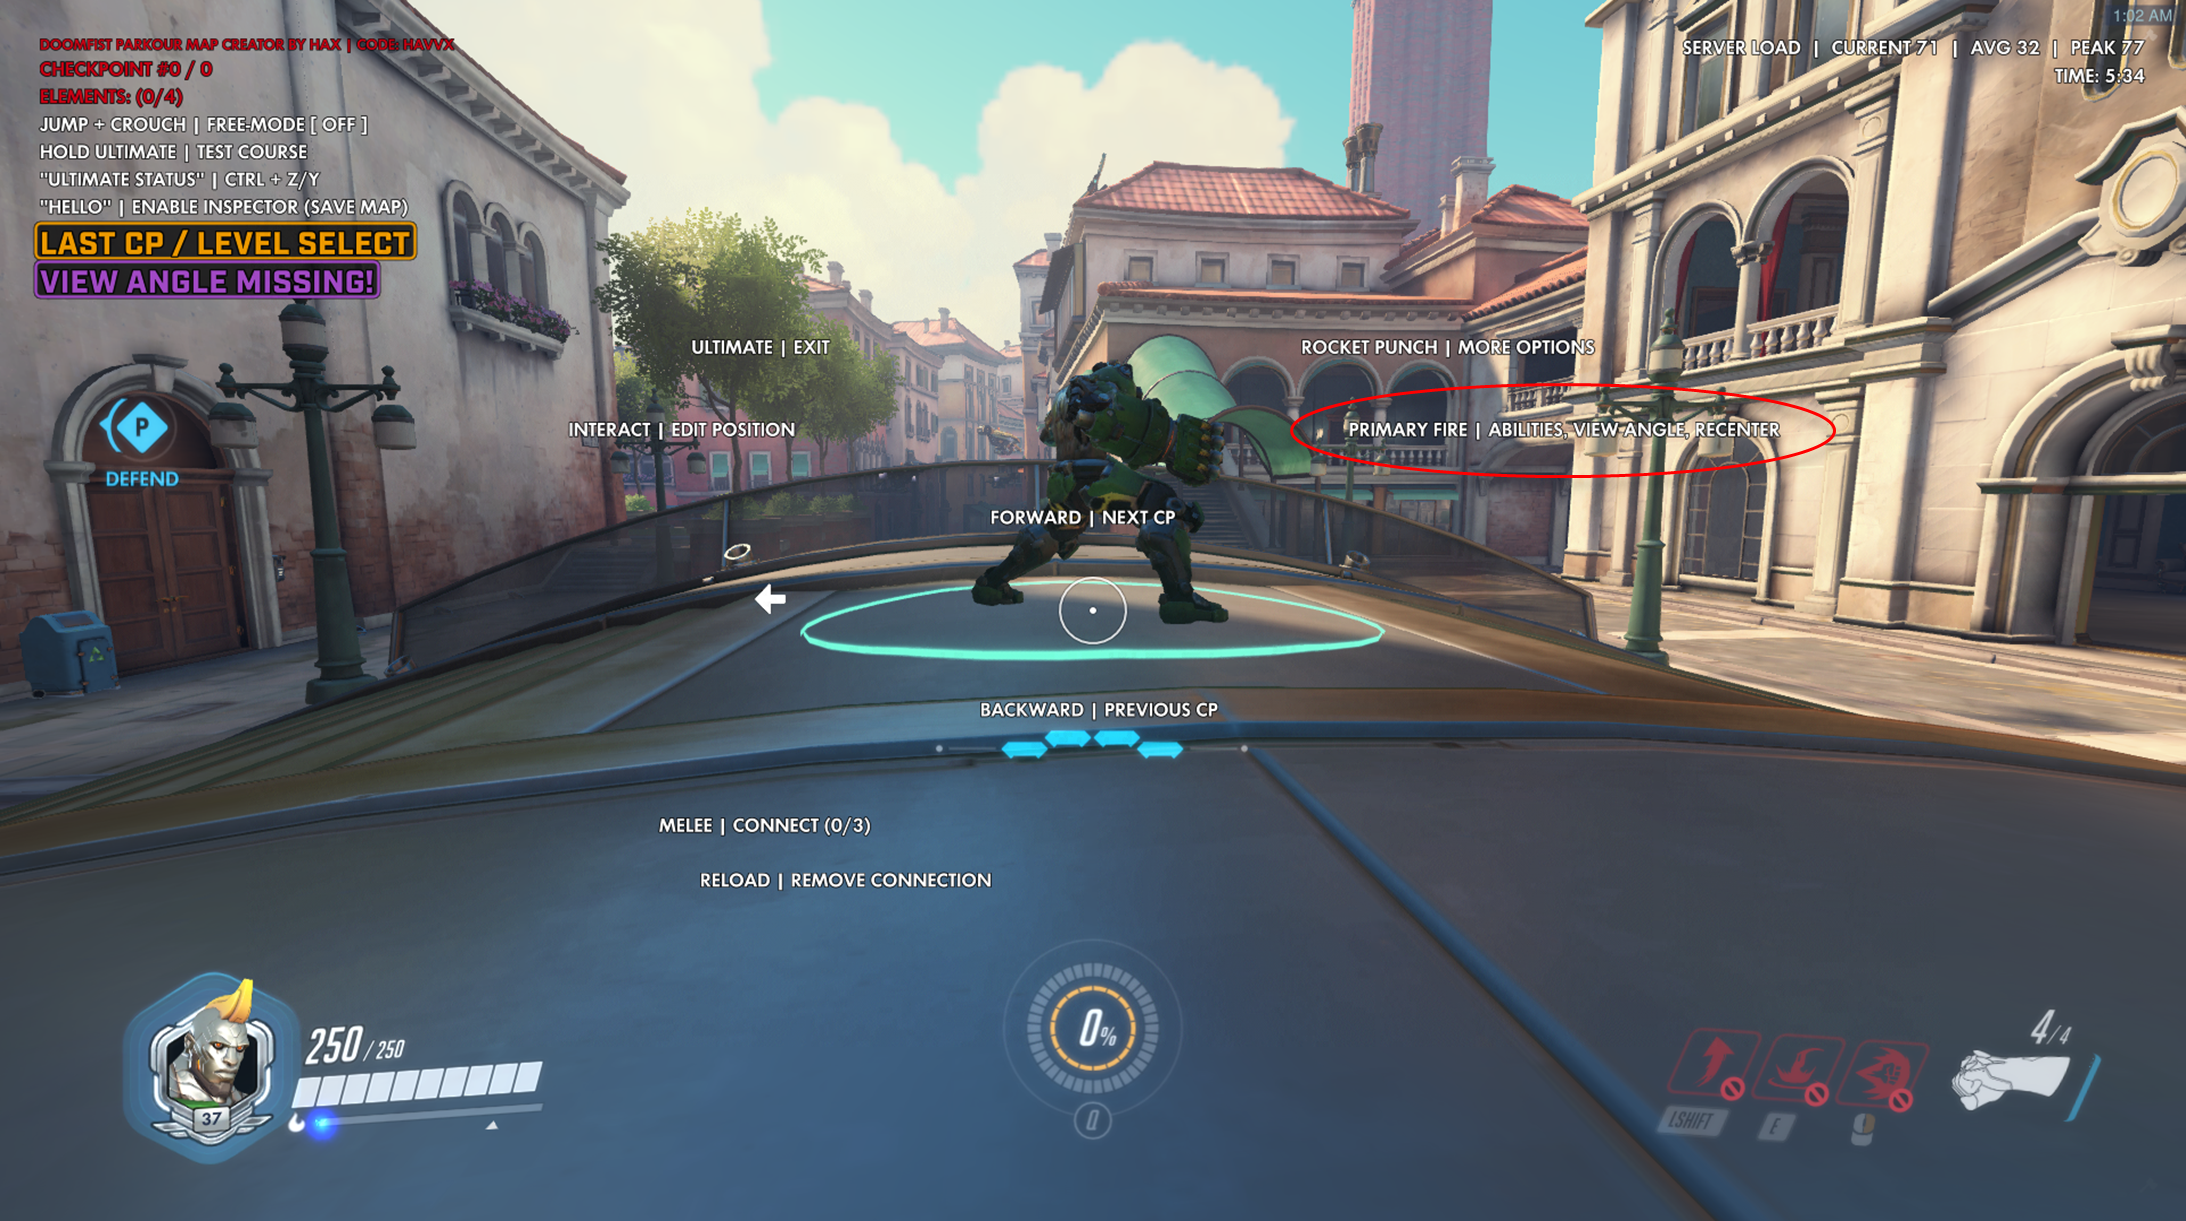
\includegraphics[width=\textwidth,height=\textheight,keepaspectratio]{Picture7.png}
            \caption{Ability enable/disable and View Angle menu button}
            \label{fig:Picture7}
        \end{figure}
    
        \begin{figure}[ht]
            \centering
            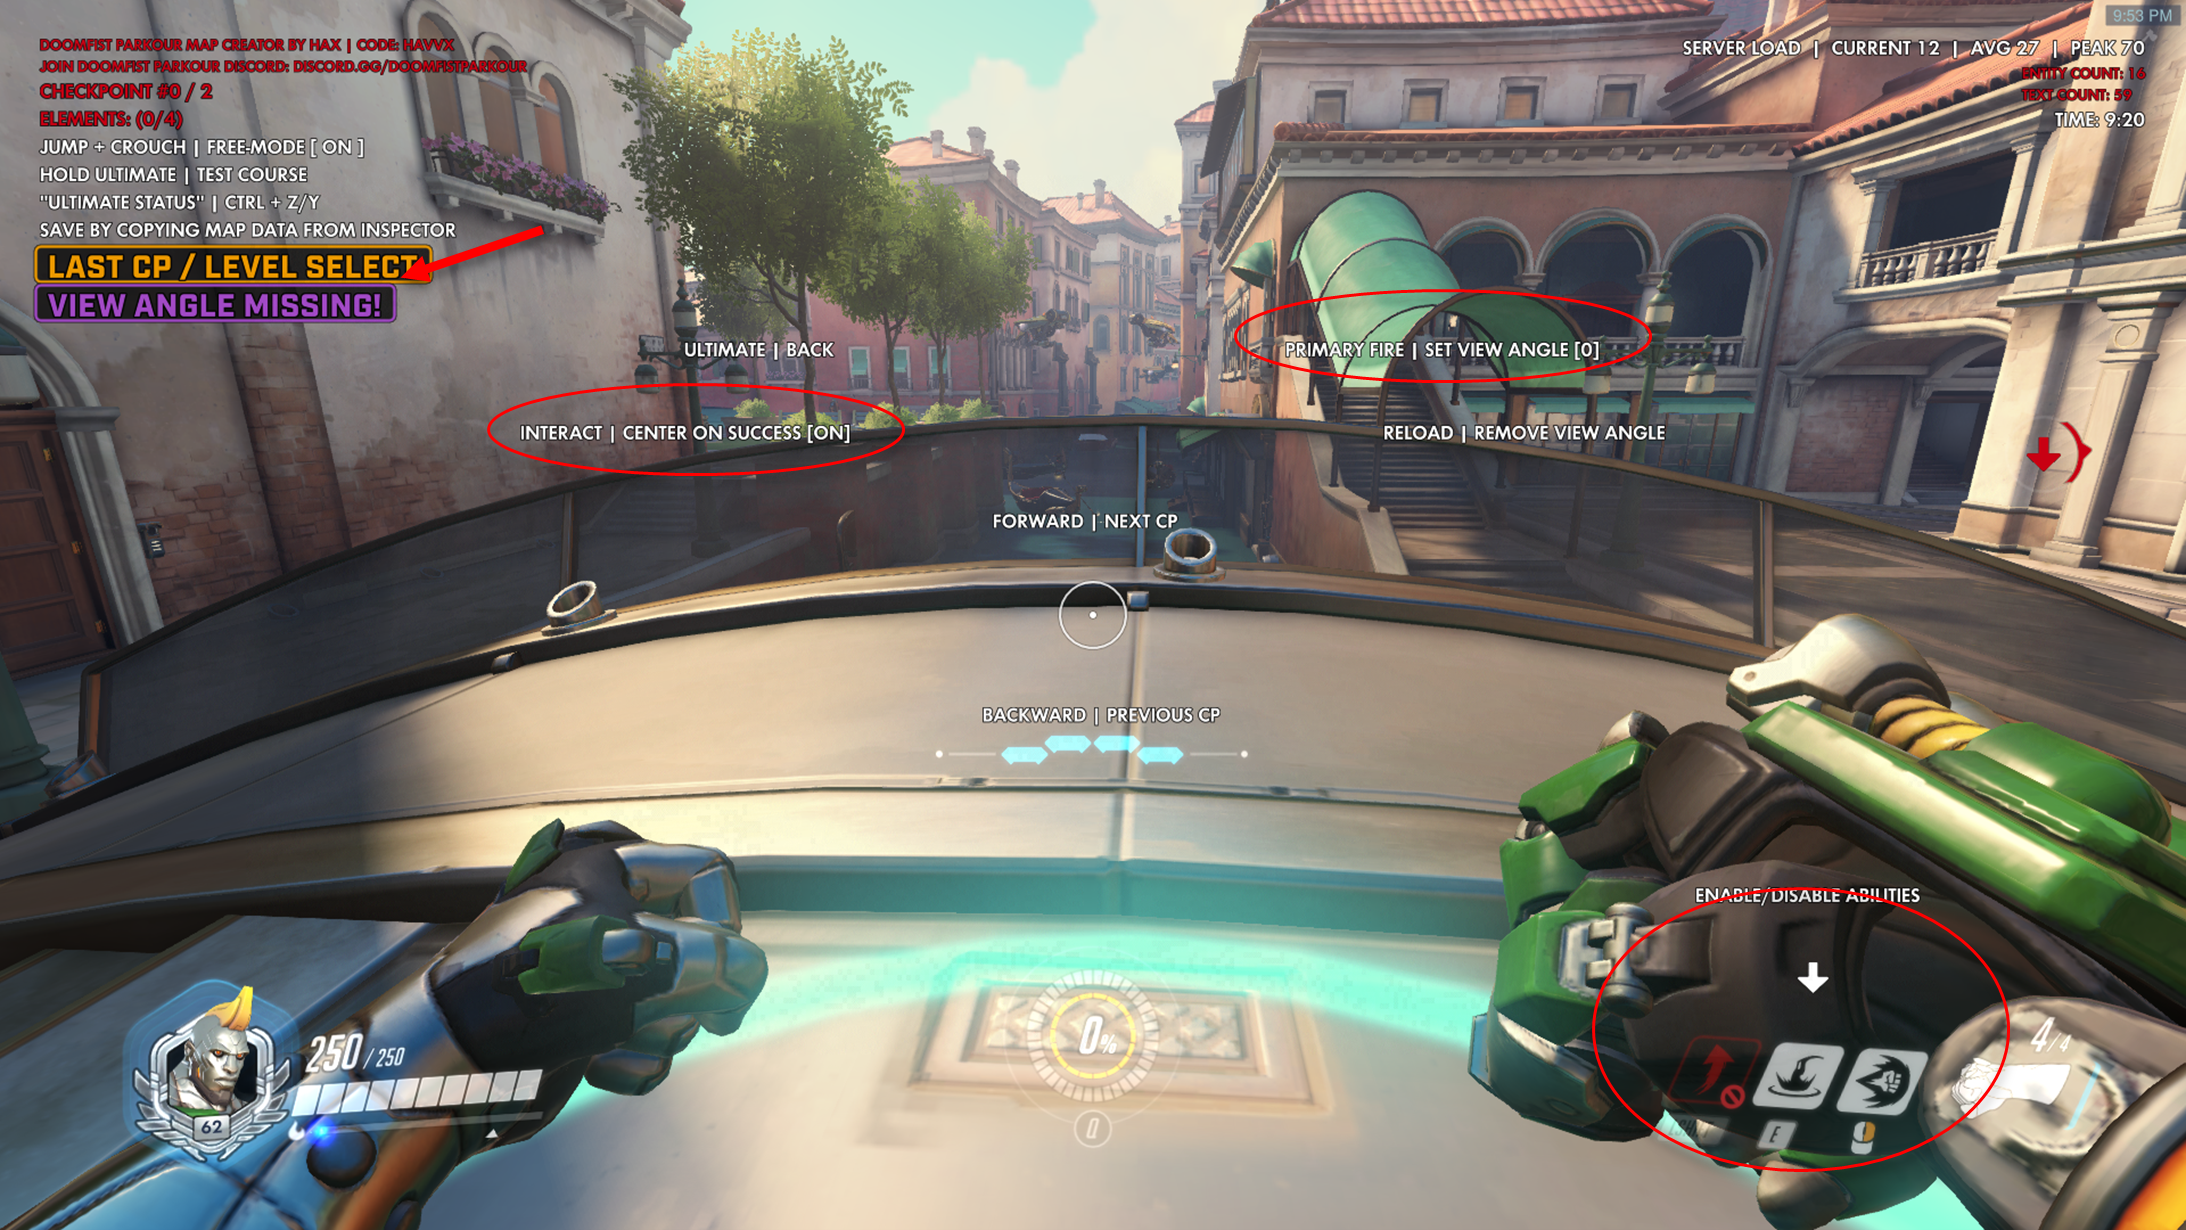
\includegraphics[width=\textwidth,height=\textheight,keepaspectratio]{Picture8.png}
            \caption{Center on Success and Set View Angle buttons}
            \label{fig:Picture8}
        \end{figure}
        \clearpage
    
        \subsubsection{View Angles}
        
            To face a precise direction after every respawn, press \keys{PRIMARY FIRE} 
            to set the view angle (\cref{fig:Picture8}, top right portion of framework menu). This will improve overall user experience.
            If this is not set, you will have to keep turning your mouse every
            time you respawn because you will end up facing a wall, the sky/floor, or some other arbitrary place. 
            Setting view angles is important for implicit hints for checkpoint routes or locations of hard to spot ability orbs.
            
            \emph{It is recommended to avoid setting a view angle on the initial level select checkpoint.}
            
            If you want to remove the view angle, you can press \keys{RELOAD} to remove it entirely. 
            After setting the view angle, the \emph{VIEW ANGLE MISSING} message in purple at the top left-hand corner of the screen will be gone. 
            This message serves as a reminder in case you sometimes forget to set the view angle. 
    
        \subsubsection{Center on Success}
            
            If you press \keys{INTERACT} (\cref{fig:Picture8}, bottom left of the framework menu), you will 
            toggle on/off the option for \emph{Center on Success}. Turning this setting off will remove the teleport to the center of the checkpoint upon successfully completing it. It is best to leave this option enabled unless you know what you are doing. This is a checkpoint-by-checkpoint \emph{Centerless} feature as seen in \emph{Pro-Mode}, which will be discussed later.
            
    \subsection{Creating a New Level or Checkpoint}
    
\end{document}
